\documentclass{beamer}

%%%%% ===== 设置主题 *****
\usetheme{Berlin}
% 可供选择的主题参见 beameruserguide.pdf
% 无导航条的主题: Bergen, Boadilla, Madrid, CambridgeUS,
%                 GoettingenAnnArbor,Pittsburgh, Rochester;
% 有树形导航条的主题: Antibes, JuanLesPins, Montpellier;
% 有目录竖条的主题: Berkeley, PaloAlto, Goettingen, Marburg, Hannover;
% 有圆点导航条的主题: Berlin, Ilmenau, Dresden, Darmstadt, Frankfurt, Singapore, Szeged;
% 有节与小节导航条的主题: Copenhagen, Luebeck, Warsaw

\useinnertheme{circles}
\useoutertheme{infolines}
\usefonttheme[onlymath]{serif}
\setbeamertemplate{navigation symbols}{} % remove the navigation
\setbeamersize{text margin left=0.8cm, text margin right=0.8cm}
\setbeamerfont{frametitle}{size=\large}
\setbeamerfont{footline}{family=\ttfamily}\setbeamertemplate{caption}[numbered]
%%%%% ===== 宏包 *****
\usepackage{amsmath,amssymb,amsfonts,ragged2e}
\usepackage{graphicx,xcolor}
\usepackage{hyperref}
\usepackage{bm}
\usepackage{amsthm}
\usepackage{ulem}
\usepackage{multirow}
% \usepackage{xeCJK}
% \usepackage{algorithmicx,algorithm}
\usepackage[linesnumbered,ruled,vlined]{algorithm2e}
\usepackage[backend=bibtex,style=numeric,sorting=none]{biblatex}
\addbibresource{reference.bib}
\setbeamerfont{footnote}{size=\tiny}
\renewcommand{\baselinestretch}{1.1}
\usepackage{ctex}
% \setCJKfamilyfont{myfont}{STSong}
% \newcommand{\MyFont}{\CJKfamily{myfont}}
%%%%% ===== 自定义命令 *****
\newcommand{\myem}[1]{\textcolor{blue}{#1}}
\renewcommand{\today}{\number\year 年\number\month 月\number\day 日}
\renewcommand{\figurename}{图}
\renewcommand{\tablename}{表}
\setbeamerfont{caption}{size=\footnotesize}
%\newtheorem{theorem}{Theorem}

\begin{document}
\justifying
\title[一种混合整数双层规划问题求解算法研究]%
{一种混合整数双层规划问题求解算法研究}

\author[杜洪博]%
{报告人: 杜洪博\\
导\quad 师: 寇彩霞\rule[0pt]{0pt}{20pt}\\}

\institute[BUPT]{\textcolor[rgb]{0.0,0.0,0.10}%
{\small\ttfamily 北京邮电大学\ 理学院\\[10pt]}}

\date{\today}

% ===== title page ====================================
\begin{frame}[plain]
	\titlepage
\end{frame}

\begin{frame}
	\frametitle{目录}
	\tableofcontents[hideallsubsections] %[pausesections]
\end{frame}

\AtBeginSection[] % Do nothing for \section*
{ \begin{frame}<beamer> %\frametitle{Outline}
		\tableofcontents[currentsection,hideallsubsections]%,currentsubsection]
	\end{frame}
}

%===== Main part start here ==========================
% 双层规划问题介绍
% 问题背景
% 混合整数双层规划问题的求解算法
% 数值实验
% 未来工作安排

\section{双层规划问题}

\begin{frame}
	\frametitle{双层规划问题的标准形式} 
	\begin{equation}
		\begin{aligned}
			\min_{x,y}& F(x,y)  \\
			&G(x,y)\leq0 \\
			&y\in\arg\operatorname*{min}_{y^{\prime}}\{f(x,y^{\prime}):g(x,y^{\prime})\leq0\},
		\end{aligned}
	\end{equation}
	\begin{itemize}
		\item $x$为上层变量, $y$为下层变量;
		\item $F(x,y)$和$f(x,y)$分别为上层和下层的目标函数;
		\item $G(x,y)$和$g(x,y)$分别为上层和下层的约束条件.
	\end{itemize}
\end{frame}

\begin{frame}
	\frametitle{双层规划问题的求解方法}
	\begin{itemize}
		\item 通过将下层问题的最优解$y$代入上层问题, 将双层规划问题转化为单层规划问题;
		
		\item KKT条件、罚函数法、信赖域法以及启发式方法等\footfullcite{sinha_review_2018}.
	\end{itemize}
\end{frame}


\section{问题背景}

\begin{frame}
	\frametitle{问题背景} 
	在多能互补电力系统优化问题中需要同时考虑系统经济性和供电稳定性,由于新能源天然的不稳定性,所以这两个目标之间存在着矛盾,为了刻画该问题,可以将其建模为混合整数双层规划问题。
	\begin{figure}
		\centering
		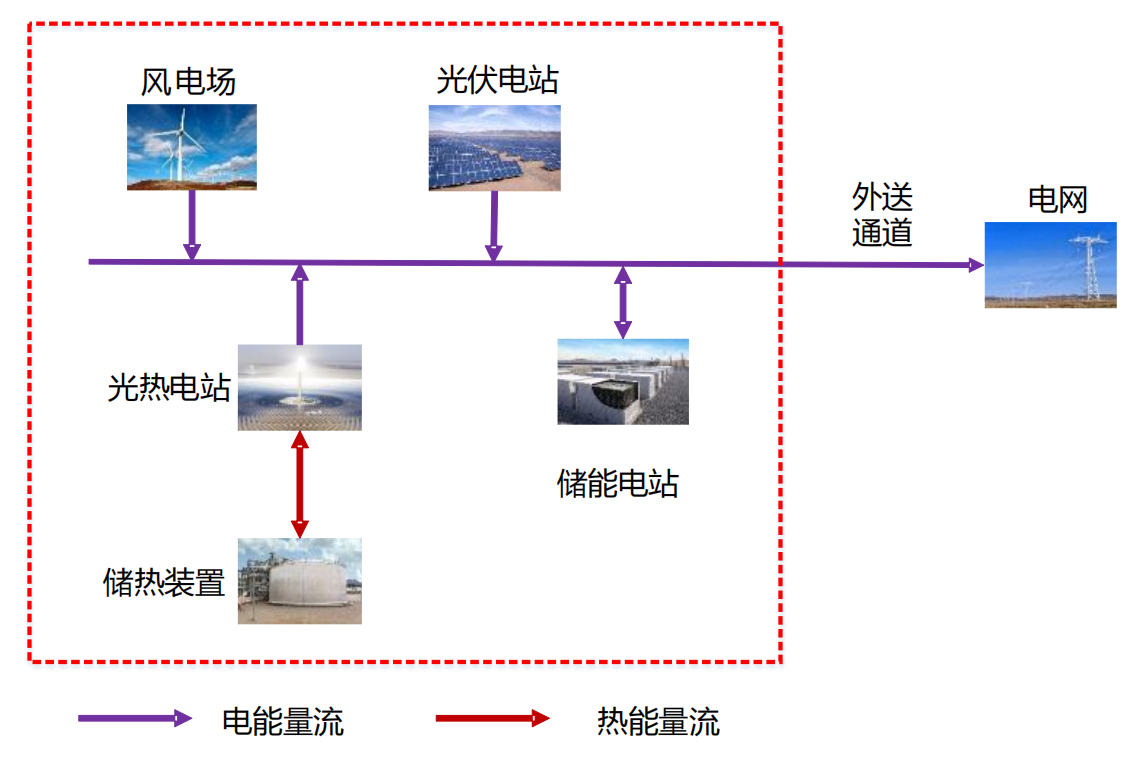
\includegraphics[width=0.6\textwidth]{pic/系统结构示意图.png}
		\caption{系统示意图}
	\end{figure}
\end{frame}

\section{一种混合整数双层规划问题求解算法} 

\begin{frame}
	Fischetti, M., Ljubić, I., Monaci, M. et al. On the use of intersection cuts for bilevel optimization. Math. Program. 172, 77–103 (2018). https://doi.org/10.1007/s10107-017-1189-5
\end{frame}

\begin{frame}

\end{frame}

\begin{frame}
	\frametitle{研究现状} 

\end{frame}

\begin{frame}

\end{frame}

\begin{frame}

\end{frame}

\begin{frame}

\end{frame}

\begin{frame}

\end{frame}

\section{未来工作安排}
\begin{frame}
	\frametitle{未来工作安排} 
	1. 继续学习文献中的方法;

	2. 实现算法并进行初步数值实验;

	3. 根据电力系统优化模型的特点, 结合分解或割平面等方法进一步提高计算效率。
\end{frame}

% ====== End =========================================
\begin{frame}
	\vspace{1em}
	\centering
	\textcolor{black}{\LARGE\bf 谢谢各位老师和同学!}

\end{frame}

\end{document}
